\documentclass[journal]{IEEEtran}

\usepackage{amsmath,amssymb,caption,comment,enumitem,float,graphicx,microtype}
\usepackage[utf8]{inputenc}
\usepackage[T1]{fontenc}
\usepackage[margin=1in]{geometry}
\usepackage{setspace}
\usepackage{fancyhdr}
\usepackage{bm}
\pagestyle{fancy}
\fancyhf{}
\rhead{\today}

\newcommand{\N}{{\mathbb N}}
\newcommand{\Z}{{\mathbb Z}}
\newcommand{\Q}{{\mathbb Q}}
\newcommand{\R}{{\mathbb R}}
\newcommand{\C}{{\mathbb C}}
\newcommand{\F}{{\mathbb F}}
\newcommand{\E}{{\mathbb E}}
\mathchardef\hyphen="2D

\title{6.867 Homework 1}
\author{Anonymous Authors}

\begin{document}

\maketitle
\thispagestyle{fancy}

\section{Implementing Gradient Descent}

\section{Linear Basis Function Regression}

\subsection{Closed-form Solution with Polynomial Basis}
% Replicate plots
Consider the basis function $$\Phi_M(x) = [\phi_0(x), \dots, \phi_M(x)],$$ where $\phi_k(x) = x^k$. Applying $\Phi_M$ to $\mathbf{X}$ gives the desired basis change, so we have the generalized linear model $$\mathbf Y = \Phi_M(\mathbf X) \cdot \bm \beta + \bm \epsilon,$$ which has the close-form solution $$\hat{\bm \beta} = (\Phi_M(\mathbf X)^T \Phi_M(\mathbf X))^{-1} \Phi_M(\mathbf X)^T \mathbf Y,$$
where $\hat{\bm \beta}$ is the maximum-likelihood estimator of the regression coefficients.

We ran regressions on the data using a few different degrees $(M = 0, 1, 3, 10)$.\footnotemark\ Below are plots of the resulting polynomial functions, compared to the given data and the true function:

\footnotetext{See the Appendix for the numerical values of the weights.}

\begin{figure}[H]
  \centering
  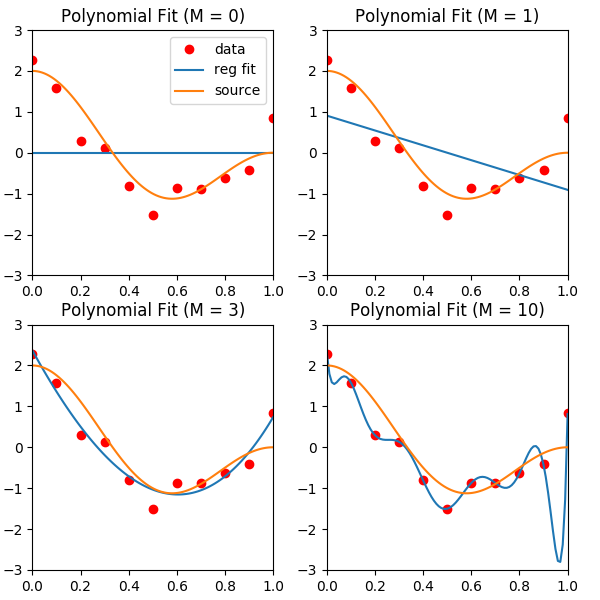
\includegraphics[width = 3.15in]{../P2/fig/part_1.png}
  \caption{M-Degree Polynomial Fit (M = 0, 1, 3, 10)}
\end{figure}

\subsection{Gradient Descent Solution with Polynomial Basis}
% Minimize SSE with Batch GD and SGD
% smallers thresholds produces slightly better fits when learn rate is small
% any threshold smaller than 1e-6 has similar results for learn rates we tested
% sgd is more sensitive to start point compared to bgd
% learn rate can't be too high or too low: doesn't converge when learn rate is too high, converges immediately when learn rate is too low (and when threshold is not adjusted accordingly)
% sgd is much more sensitive to learn rate as well
% stucks in local minima when degree is high -> more local minima


\subsection{Closed-form Solution with Cosine Function Basis}

\section{Ridge Regression}

\section{Sparsity and Lasso}

\section{Appendix}
% Coefficients in 2.1

\end{document}